\chapter{Modeling techniques for SAF microarchitectures}
\label{chapter:modeling}

Recall that assigning analytical models to SAF microarchitecture primitives is important in order to enable evaluation and comparison of designs. This section will introduce the overarching modeling strategy employed in this work, tying together energy, area and workload modeling into a single scheme. The following considerations are relevant:

\begin{itemize}
    \item Recall from Chapter~\ref{chapter:conceptual_framework} that one of the goals of this work is to associate SAF microarchitecture primitives with analytical cost models (i.e. models of energy and area.) Toward that end, Chapter~\ref{chapter:rtl} introduced a number of RTL designs which were developed and characterized for this work.
    \item However, we still need a way to convert RTL characterization results, into SAF microarchitecture primitive models with well-defined energy-per-action and area.
    \item Also recall from Chapter~\ref{chapter:conceptual_framework} that another goal of this work is to decouple SAF microarchitecture from architecture and dataflow. As shown in Figure~\ref{fig:sparse_sbuff_wkld_overview}, we hope to encapsulate all details of architecture and dataflow behind format interfaces with well-defined measures of workload.
\end{itemize}

Recall that the RTL in Chapter~\ref{chapter:rtl} is parameterized. The power-consumption and area of RTL components will scale with the parameter values. However, more subtly, the \textit{load-handling capability} of the RTL components also scales with the parameter values. For example, a naive two-finger-merge-based intersection unit will be able to intersect more input operands per cycle, if it is constructed with a greater degree of input vectorization; or, a prefix sum unit designed for operands which have some number of bits, will be able to support operands with a larger range of possible values if the number of bits is increased. Thus RTL parameters represent a tradeoff between cost (power, area) and load-handling capability.

The motivation for assigning a measure of workload to each format interface at the outset, is so that the scale parameters of the SAF microarchitecture may be tuned properly. The SAF microarchitecture scale parameters should be set such that

\begin{itemize}
    \item The SAF microarchitecture can process sparse format metadata at the rate which it is being served over the format interface by the smartbuffer.
    \item The SAF microarchitecture is capable of serving processed outputs back to the buffer via the format interface, at the rate which the buffer was designed for.
\end{itemize}

Failure to meet either of the above requirements should in principle lead to a slowdown in the whole design.

\section{Load modeling}

This section describes a multi-dimensional measure of the load that architectural buffers and arithmetic units impose on SAF microarchitectures. The area and action-energy of each SAF microarchitecture will scale as a function of load-handling requirements; having a way to quantify loading will allow us to solve for RTL parameters that minimize cost while meeting load handling requirements.

On first blush, it might seem appropriate to use a single scalar quantity to characterize both load and load-handling capability of a component. For example, the \textit{throughput} (number of inputs processed per time) would seem like a good candidate for measuring load and load-handling requirements (since FLOPs is a common compute performance metric.)

However, it quickly becomes apparent that load and load-handling ability are multi-dimensional; what follows is a list of factors which influence loading and load-handling requirements:

\begin{itemize}
    \item \textbf{Word-width.} A microarchitecture capable of handling the throughput imposed by some workload, may nonetheless be unsuitable if i.e. the microarchitecture is expected to process sparse format metadata possessing a greater bitwidth than what the microarchitecture was designed for. Thus, word-width is a dimension of load, and the upper limit on word-width is a dimension of load-handling capability for a particular component.
    \item \textbf{Size of abstract dense rank which underlies a sparse fiber.} Consider a bitmask intersection unit, as employed in the SparTen accelerator paper \cite{sparten}. The degree of parallelism of the bitmask intersection unit microarchitecture is not a function of the throughput of metadata nor of the number of bits in a metadata word (which is in fact equal to one for bitmask format), but rather the parallelism must meet or exceed the cardinality of the abstract dense ranks which underly the sparse fibers being intersected. Thus, the cardinality of the dense rank which underlies a sparse fiber is a dimension of the load on the microarchitecture. The parallelism of the bitmask intersection unit exemplifies a dimension of the microarchitecture's load-handling capability, specifically an upper-limit on dense rank cardinality which the microarchitecture can handle.
    \item \textbf{Memory access width.} The SAF microarchitecture must be able to receive sparse format metadata in chunks equal to the memory's access bitwidth - i.e., for metadata with a bitwidth of 4 stored in a memory with 8-bit-wide reads, up to two metadata words may be made available to the SAF microarchitecture per access, worst-case. If the SAF microarchitecture only needs to read format metadata a few times over many cycles, then the latency of sequentially processing multiple metadata words can be hidden inside the time between wide reads. However, a SAF microarchitecture that is making wide memory accesses every cycle cannot hide the latency of sequential processing and thus requires a (probably more costly) SIMD design. This motivates memory access width as a dimension of load and load-handling capability.
    \item \textbf{Local architectural throughput.} Suppose that an architecture uses a SIMD MAC unit capable of 4x $C = C + A \times B$ operations per cycle to compute an inner-product; let's define $4$ MACs/cycle as the \textit{arithmetic throughput requirement.} To avoid MAC underutilization, the arithmetic throughput requirement in turn poses requirements on the whole design; for example, four $A$ and four $B$ operands per cycle are read from the $A$ and $B$ buffers respectively. 

    % Radix-2 intersection example figure
    \begin{figure}[H]
        \centering
        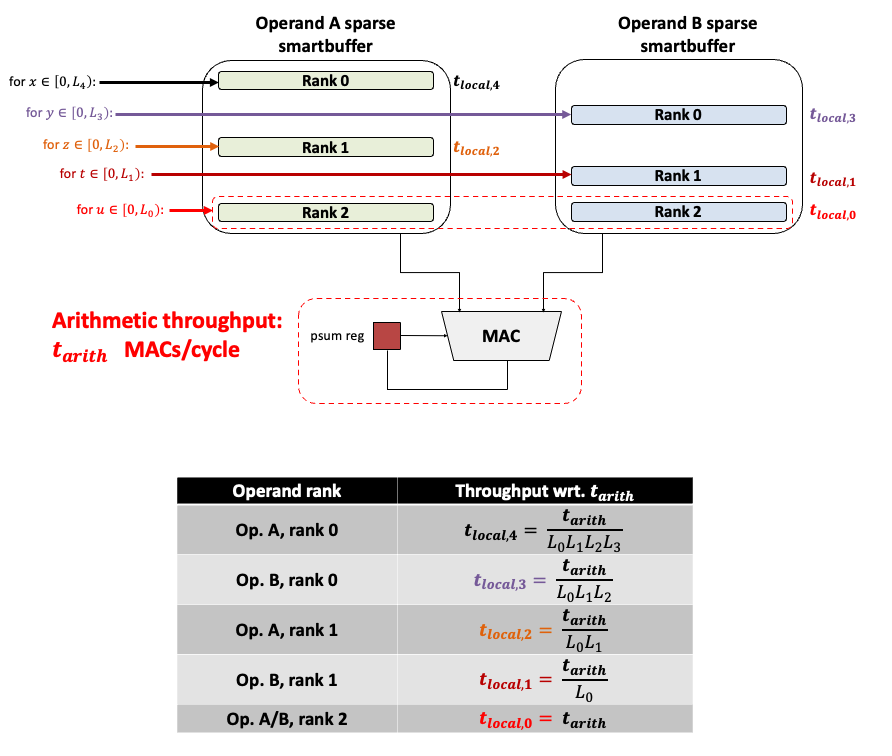
\includegraphics[width=\linewidth]{figures/local_throughput_diagram.png}
        \caption{The local throughput at each rank grows with increasing arithmetic throughput, and shrinks in proportion to the stride of the loop(s) which the fiber is bound to.}
        \label{fig:local_throughput_diagram}
    \end{figure}

    As an optimization, the designer implements a bidirectional skipping SAF between buffers $A$ and $B$. The skipping microarchitecture intersects $A$ and $B$ metadata and outputs a pair of $A$ and $B$ data read addresses for each intersection match. Consider what load-handling requirements the skipping microarchitecture must be designed for, in order to avoid MAC under-utilization: the skipping microarchitecture must serve $4$ $A$ addresses and $4$ $B$ addresses per cycle in order to facilitate reading 4 data values per cycle from each operand. Notably, this is a requirement on the skipping microarchitecture which results directly from the arithmetic throughput design-point.

    Note that in the above example, the skipping microarchitecture, buffers, and MAC are all synchronized with the innermost loop of the mapping loop-nest; this is the fastest loop. Conversely, the outermost loops of the mapping loop-nest have greater latency between loop iterations (i.e. more cycles-per-iteration). Microarchitectures synced to slower loops can maximally exploit latency-hiding to relax throughput-handling requirements by spreading out sequential processing over the time between loop iterations. Microarchitectures synced to faster loops must be capable of handling higher processing throughput without exploiting latency hiding. This state of affairs is summarized in Figure~\ref{fig:local_throughput_diagram}
    
    As a precedent, Sparseloop\cite{sparseloop} assumes that data is pre-tiled to match the loop-nest. Under this assumption there is a reasonably clean mapping from loops in the loop nest to fibers in the fibertree of an operand, and thus a microarchitecture which interacts with fiber $i$ must support the throughput imposed by the corresponding loop in the loop-nest. For example, the inner-most loop must keep pace with the arithmetic throughput-handling requirement imposed by the MAC, so any microarchitecture which interacts with the fiber(s) corresponding to the inner loop must also keep pace with the arithmetic throughput requirement. \textit{All other things being equal}, the microarchitectural throughput-handling requirement decreases monotonically as you ascend hierarchically within a fibertree, because successively higher fibers correspond to successively slower loops. 
    
    Define \textit{local architectural throughput} as the unique throughput requirement for processing a \textit{particular} fiber within a \textit{particular} buffer, owing to the synchronization of the whole architecture with the mapping loop nest. Local architecture throughput is a key dimension of the load which the architecture imposes on a SAF microarchitecture. Consequently, throughput-handling capability is a key design requirement - \textit{but not the only key requirement} - for the SAF microarchitecture.

    We can shorten local architectural throughput to ``local throughput'' or $t_{local}$.
    
    \item \textbf{Degree of fiber sparsity.} Suppose that a fiber with a bitmask representation format resides in some buffer within an architecture. The local architecture throughput requirement for processing this fiber places a lower bound on how many non-zero fiber payloads must be traversed per cycle.

    Since it is given that the fiber is subject to a bitmask format SAF optimization, a format microarchitecture is required for parsing the metadata format. Based on the programming model developed in this work, the buffer will have several format interface ports to facilitate fiber metadata processing: \textit{md\_out}, \textit{pos\_in}, \textit{at\_bound\_in}. The format microarchitecture's ports are wired to read bitmask metadata from the buffer \textit{md\_out} port, and generate an active-high signal at \textit{at\_bound\_in} to signal when the entire fiber has been processed.

    How do we derive the format microarchitecture throughput-handling requirement from the local architectural throughput requirement associated with the fiber? The local architectural throughput applies to the rate of traversing non-zero payload values within the fiber, and the number of non-zero payloads may be much less than the dense size of the abstract rank associated with the fiber. In contrast, the number of $1$-bit bitmask metadata words matches the dense rank size regardless of how many non-zero payloads the sparse fiber has. Metadata parsing by the format microarchitecture must keep pace with the traversal of non-zero payloads in the fiber, thus if the fiber is 90\% sparse/10\% dense, $10$ $1$-bit bitmask metadata words must be parsed per non-zero data value on average; if the fiber is 99\% sparse/1\% dense, $100$ $1$-bit bitmask metadata words must be parsed per non-zero data value on average.

    More generally, for a bitmask-formatted fiber with local architectural throughput requirement $t_{local}$ (in payloads/cycle) and a sparsity fraction $s$, the format microarchitecture must support a metadata parsing throughput of

    \[t_{parse} = \frac{1}{1-s}t_{local}\]

    Of course, this relationship only holds for bitmask representation format. A representation format such as coordinate-payload has one explicit-coordinate metadata value per non-zero payload, thus \[t_{parse} = t_{local}\]

    The point is, sparsity $s$ matters because it \textit{sometimes} modulates the microarchitectural throughput-handling requirement imposed by a fiber's local architectural throughput, and thus fiber sparsity is a key dimension of load.
\end{itemize}

\subsection{Workload vectors}
\label{sec:loadspaces}

To concisely and effectively model loading and load-handling capability, this work introduces the concept of \textit{workload vectors} for representing the workload imposed on a SAF microarchitecture. The dimensions of a workload vector are based on the quantities discussed in the previous section, are represented graphically in Figure~\ref{fig:workload_representation}, and are summarized in Table~\ref{table:workload_dimension_mnemonics}.

% Loadspace dimensions
\begin{figure}[H]
    \centering
    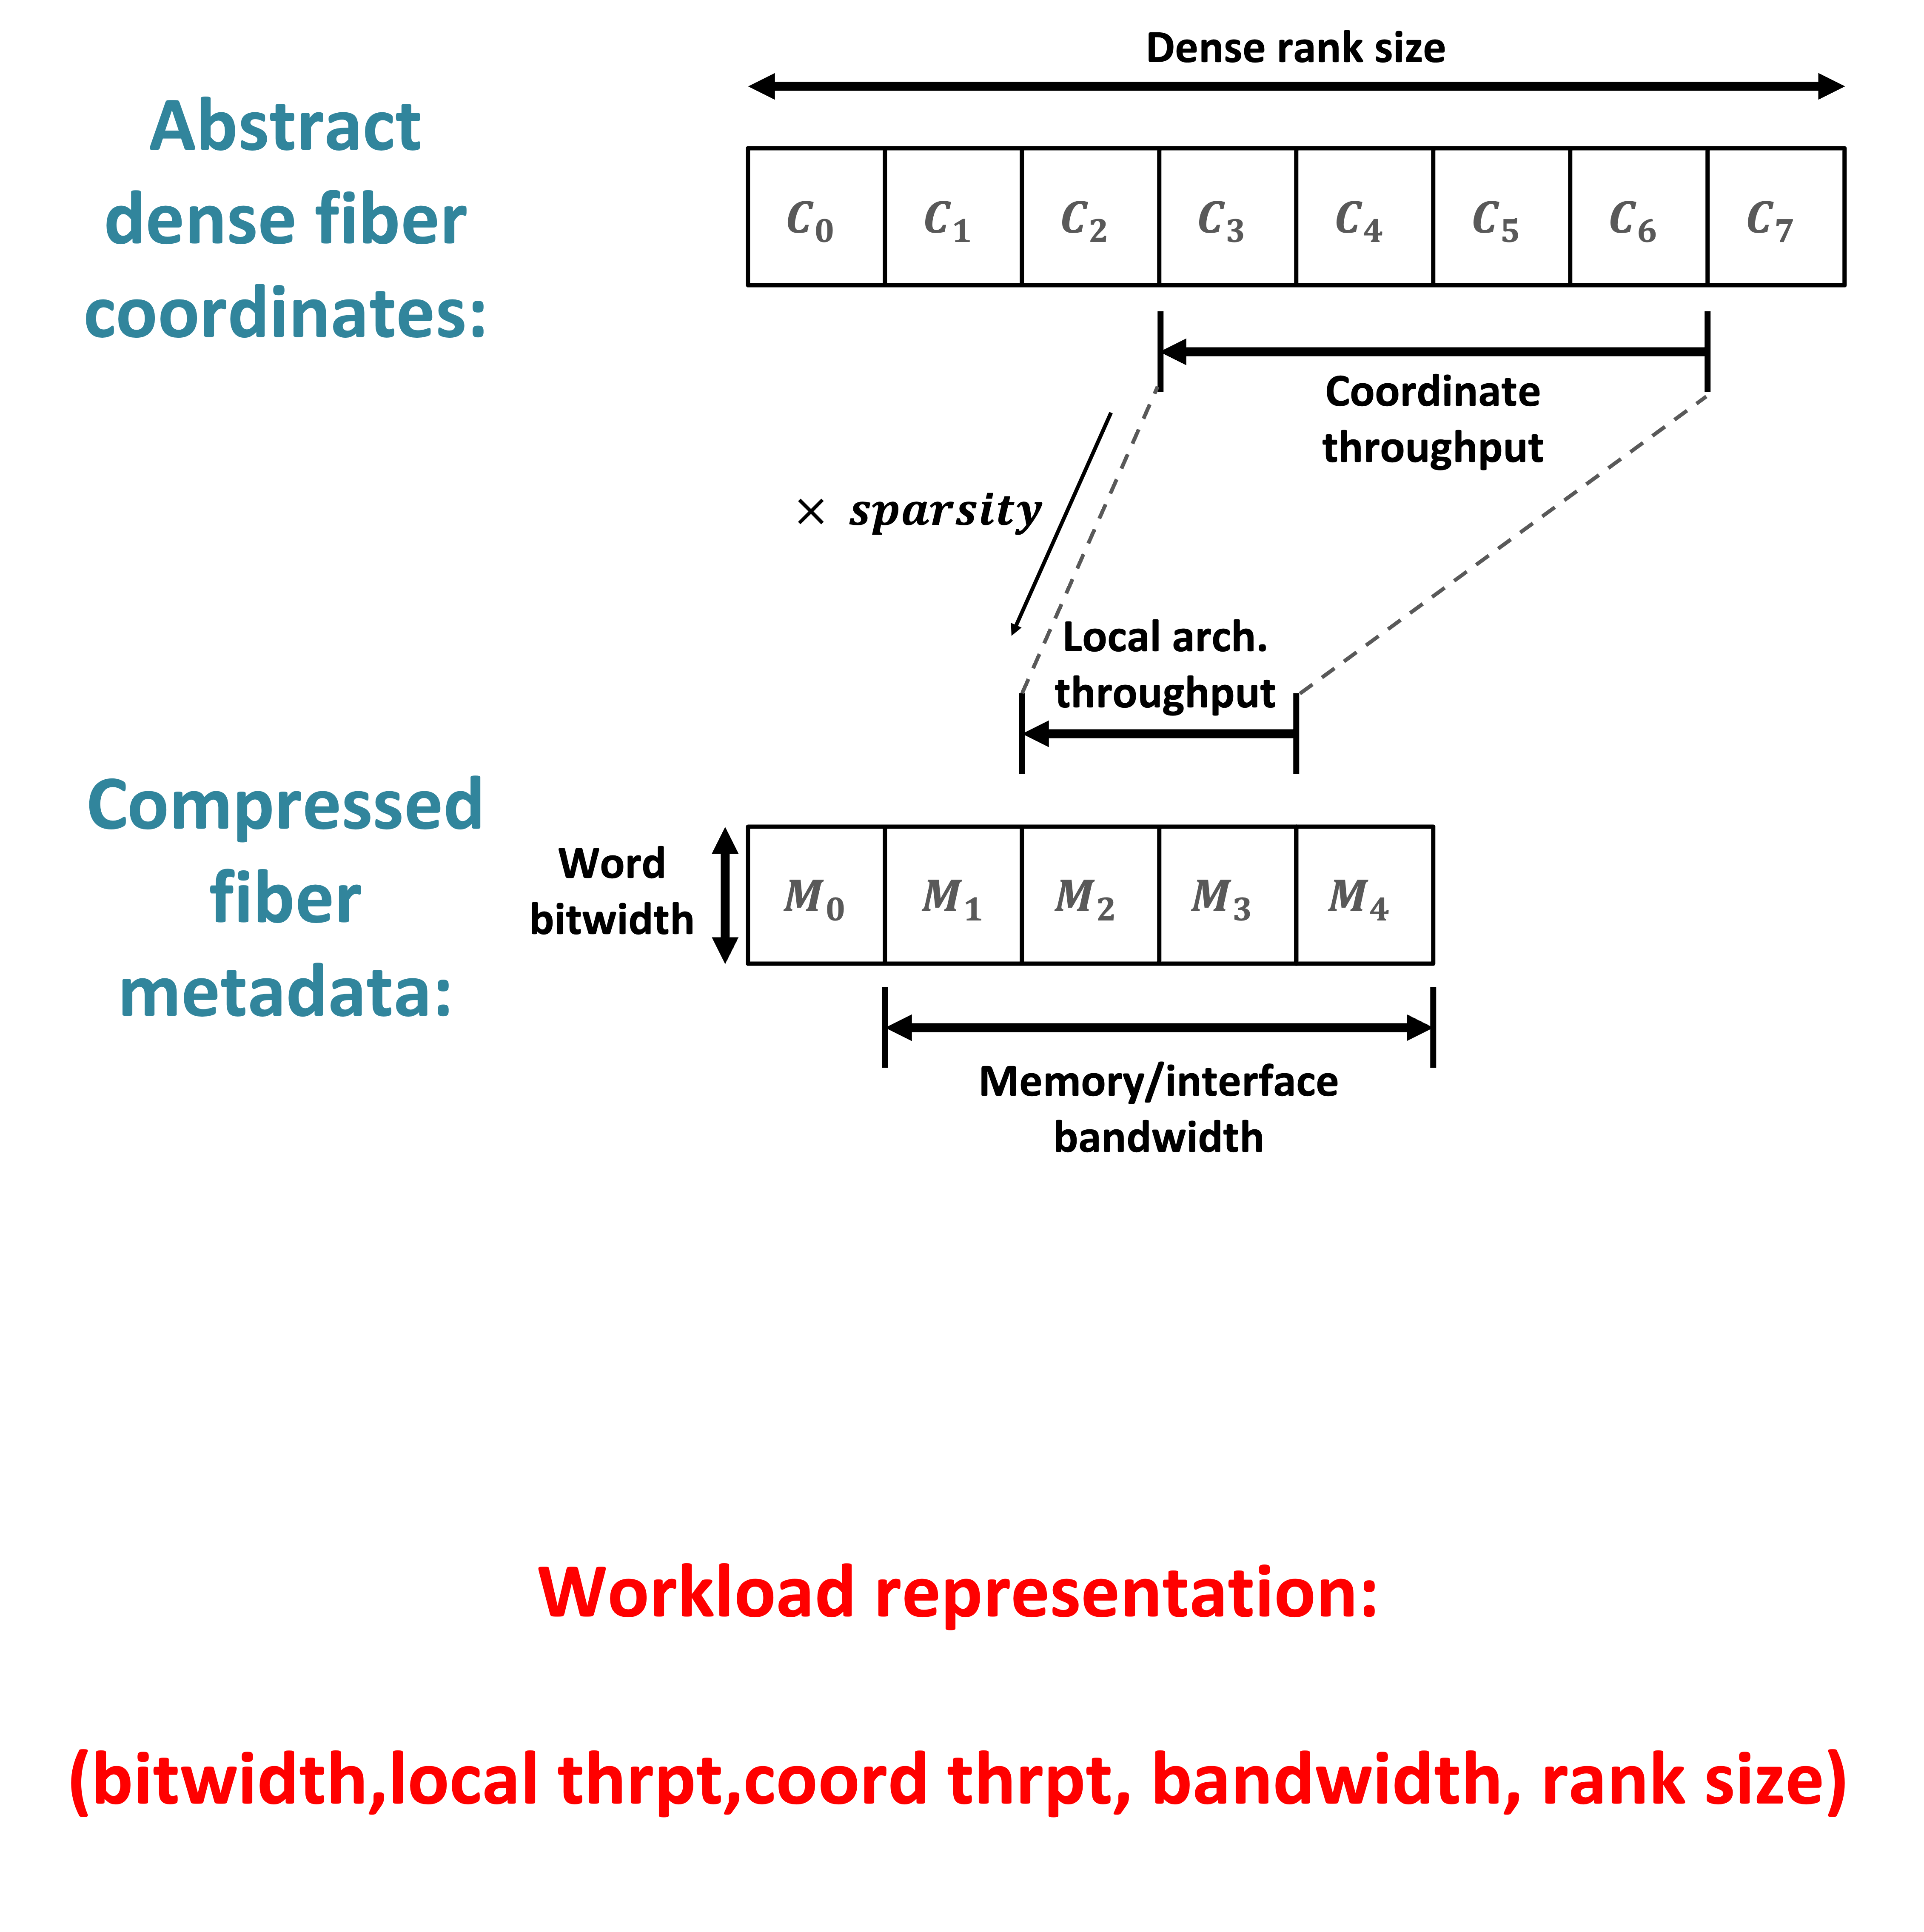
\includegraphics[width=\linewidth]{figures/workload_representation.png}
    \caption{This work proposes modeling workloads as ``workload vectors''. Here, \textit{word bitwidth},  \textit{local architectural throughput}, \textit{coordinate throughput}, and \textit{dense rank size} are proposed as key workload dimensions when designing SAF microarchitectures.}
    \label{fig:workload_representation}
\end{figure}

    \begin{table}[h]
        \centering
        \caption{Mnemonics for workload dimensions.}
        \label{table:workload_dimension_mnemonics}
        \begin{tabular}{||c|c|c|c||}
            \hline \hline
            Workload Dimension & Mnemonic & Stands for & Units \\
            \hline \hline
            Dense rank size & nc & num. coordinates & Coordinates \\
            \hline
            Local throughput & pr & position rate & Words/Cycle \\
            \hline
            Sparsity & sp & sparsity & \% \\
            \hline
            Bitwidth & ww & word width & Bits \\
            \hline
            Bandwidth & bw & read width & Bits \\
            \hline \hline
        \end{tabular}
    \end{table}

\section{Defining workload boundary conditions}

In this work, the approach to decoupling dataflow from SAF microarchitecture is to abstract dataflow behind \textit{workload boundary conditions} associated with each format interface on each sparse smartbuffer.

Recall from Figure~\ref{fig:format_interface} that a format interface is an IO bundle which allows SAF microarchitecture to interface with a tensor rank resident at some sparse smartbuffer. The wires within the format interface IO bundle (from the smartbuffer perspective) are

\begin{itemize}
    \item pos\_in - input which receives position offsets for looking up payloads.
    \item md\_out - fiber sparse format metadata output.
    \item at\_bound\_in - flag input for resetting traversal.
\end{itemize}

Suppose that the a particular format interface on some smartbuffer, is associated with a particular fibertree rank with dense rank size $nc$, sparsity $sp$, metadata word bitwidth $ww_{md}$, and position word bitwidth $ww_{pos}$. Suppose that owing to the loop nest, the rank is associated with some local architectural throughput $t_{local}$. Finally, suppose that the smartbuffer with this format interface has a read bandwidth of $rw$ bits. Each wire within the format interface IO bundle is associated with a workload boundary condition, as follows:

\begin{itemize}
    \item \textit{pos\_in:} 
    \begin{itemize}
        \item $pos\_in.pr \geq t_{local}$
        \item $pos\_in.ww = ww_{pos}$
        \item $pos\_in.nc = nc$
        \item $pos\_in.sp = sp$
        \item $pos\_in.rw = rw$
    \end{itemize}

    Notably, the constraint on $pos\_in.pr$ is required in order for the rate of payload lookups to keep pace with the loop nest; otherwise, the architecture might experience a slowdown.
    
    \item \textit{md\_out:} 

    \begin{itemize}
        \item $md\_out.pr \leq md\_out.rw/md\_out.ww$
        \item $md\_out.ww = ww_{md}$
        \item $md\_out.nc = nc$
        \item $md\_out.sp = sp$
        \item $md\_out.rw = rw$
    \end{itemize}

    The constraint of $md\_out.pr$ reflects that the format interface may not output sparse format metadata with a throughput rate exceeding the memory's read bandwidth, in words.

    \item \textit{at\_bound\_in:} 

    \begin{itemize}
        \item $at\_bound\_in.pr \leq md\_out.rw/md\_out.ww$
        \item $at\_bound\_in.ww = ww_{md}$
        \item $at\_bound\_in.nc = nc$
        \item $at\_bound\_in.sp = sp$
        \item $at\_bound\_in.rw = rw$
    \end{itemize}
\end{itemize}

\section{Specifying a SAF microarchitecture primitive model}

The previous section introduced workload vectors to describe loading; this section introduces \textit{scale parameter} vectors to describe a component's \textit{workload handling capability.} By way of introducing this concept, this section overviews the approach to specifying SAF microarchitecture primitive models.

\clearpage

\begin{figure}[H]
    \centering
    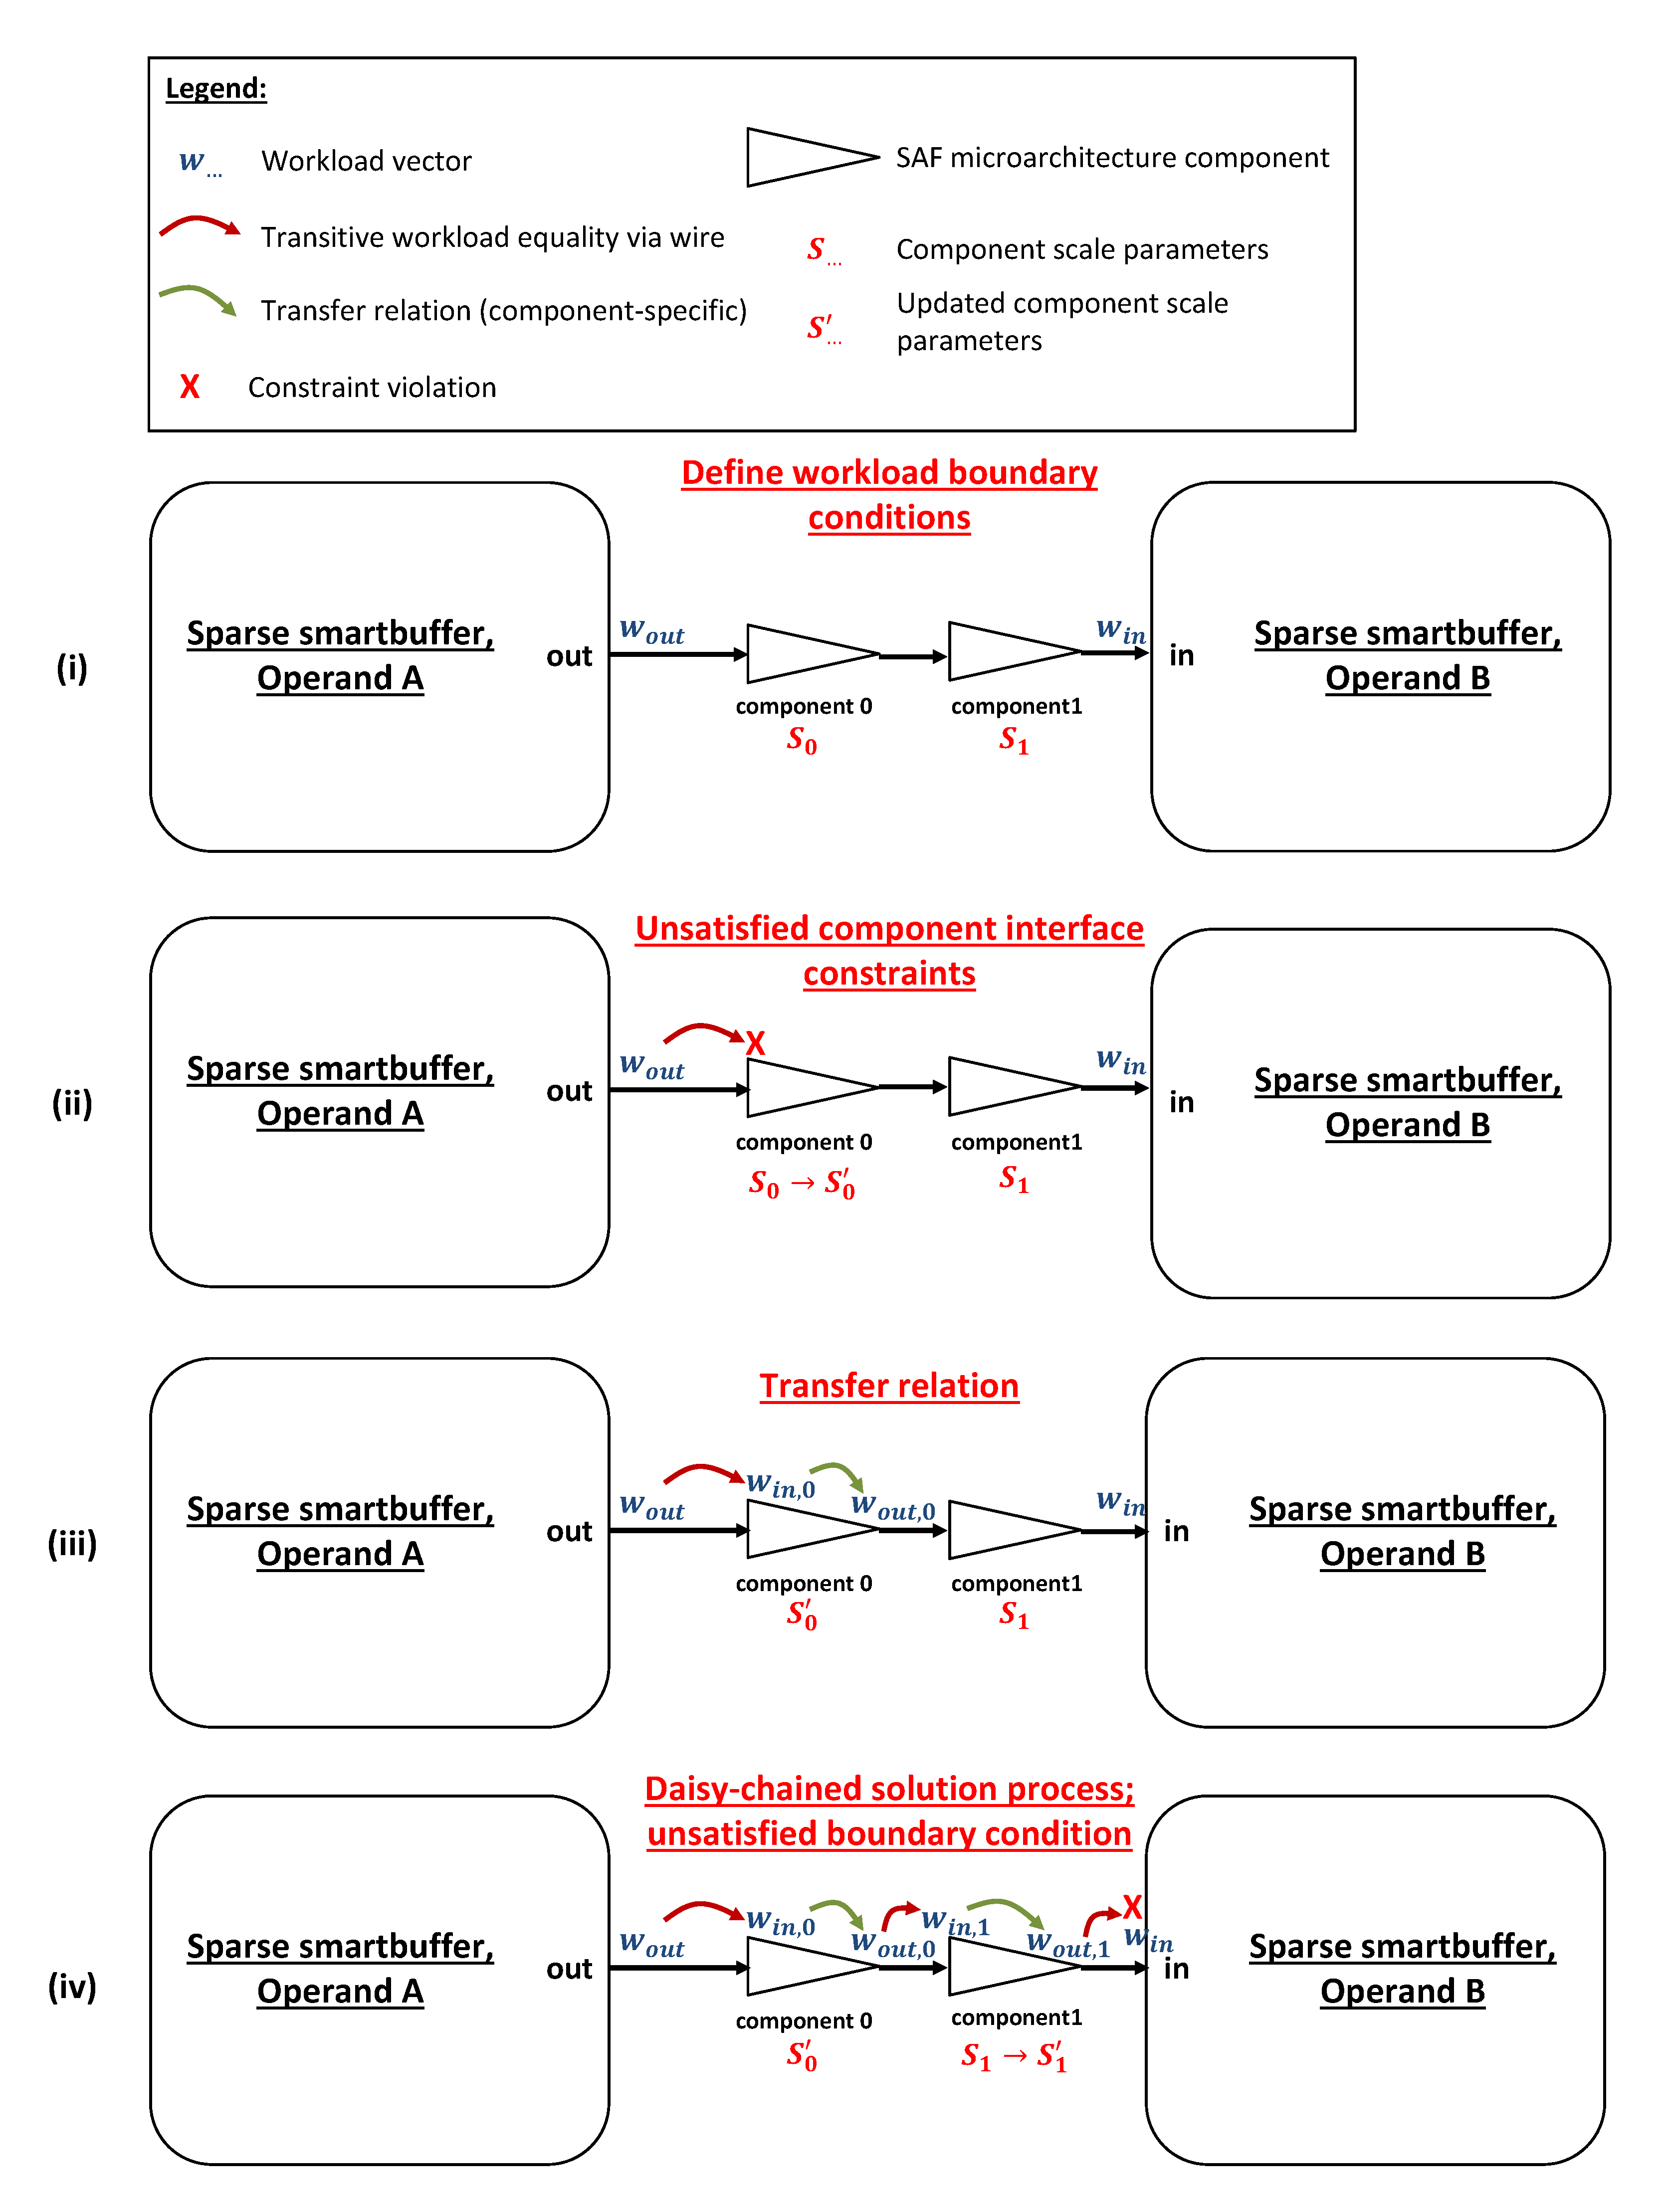
\includegraphics[width=0.8\textwidth]{figures/workload_example.pdf}
    \caption{Example of SAF microarchitecture scale inference, via daisy-chained workload solving.}
    \label{fig:workload_example}
\end{figure}

\clearpage

\begin{figure}[H]
    \centering
    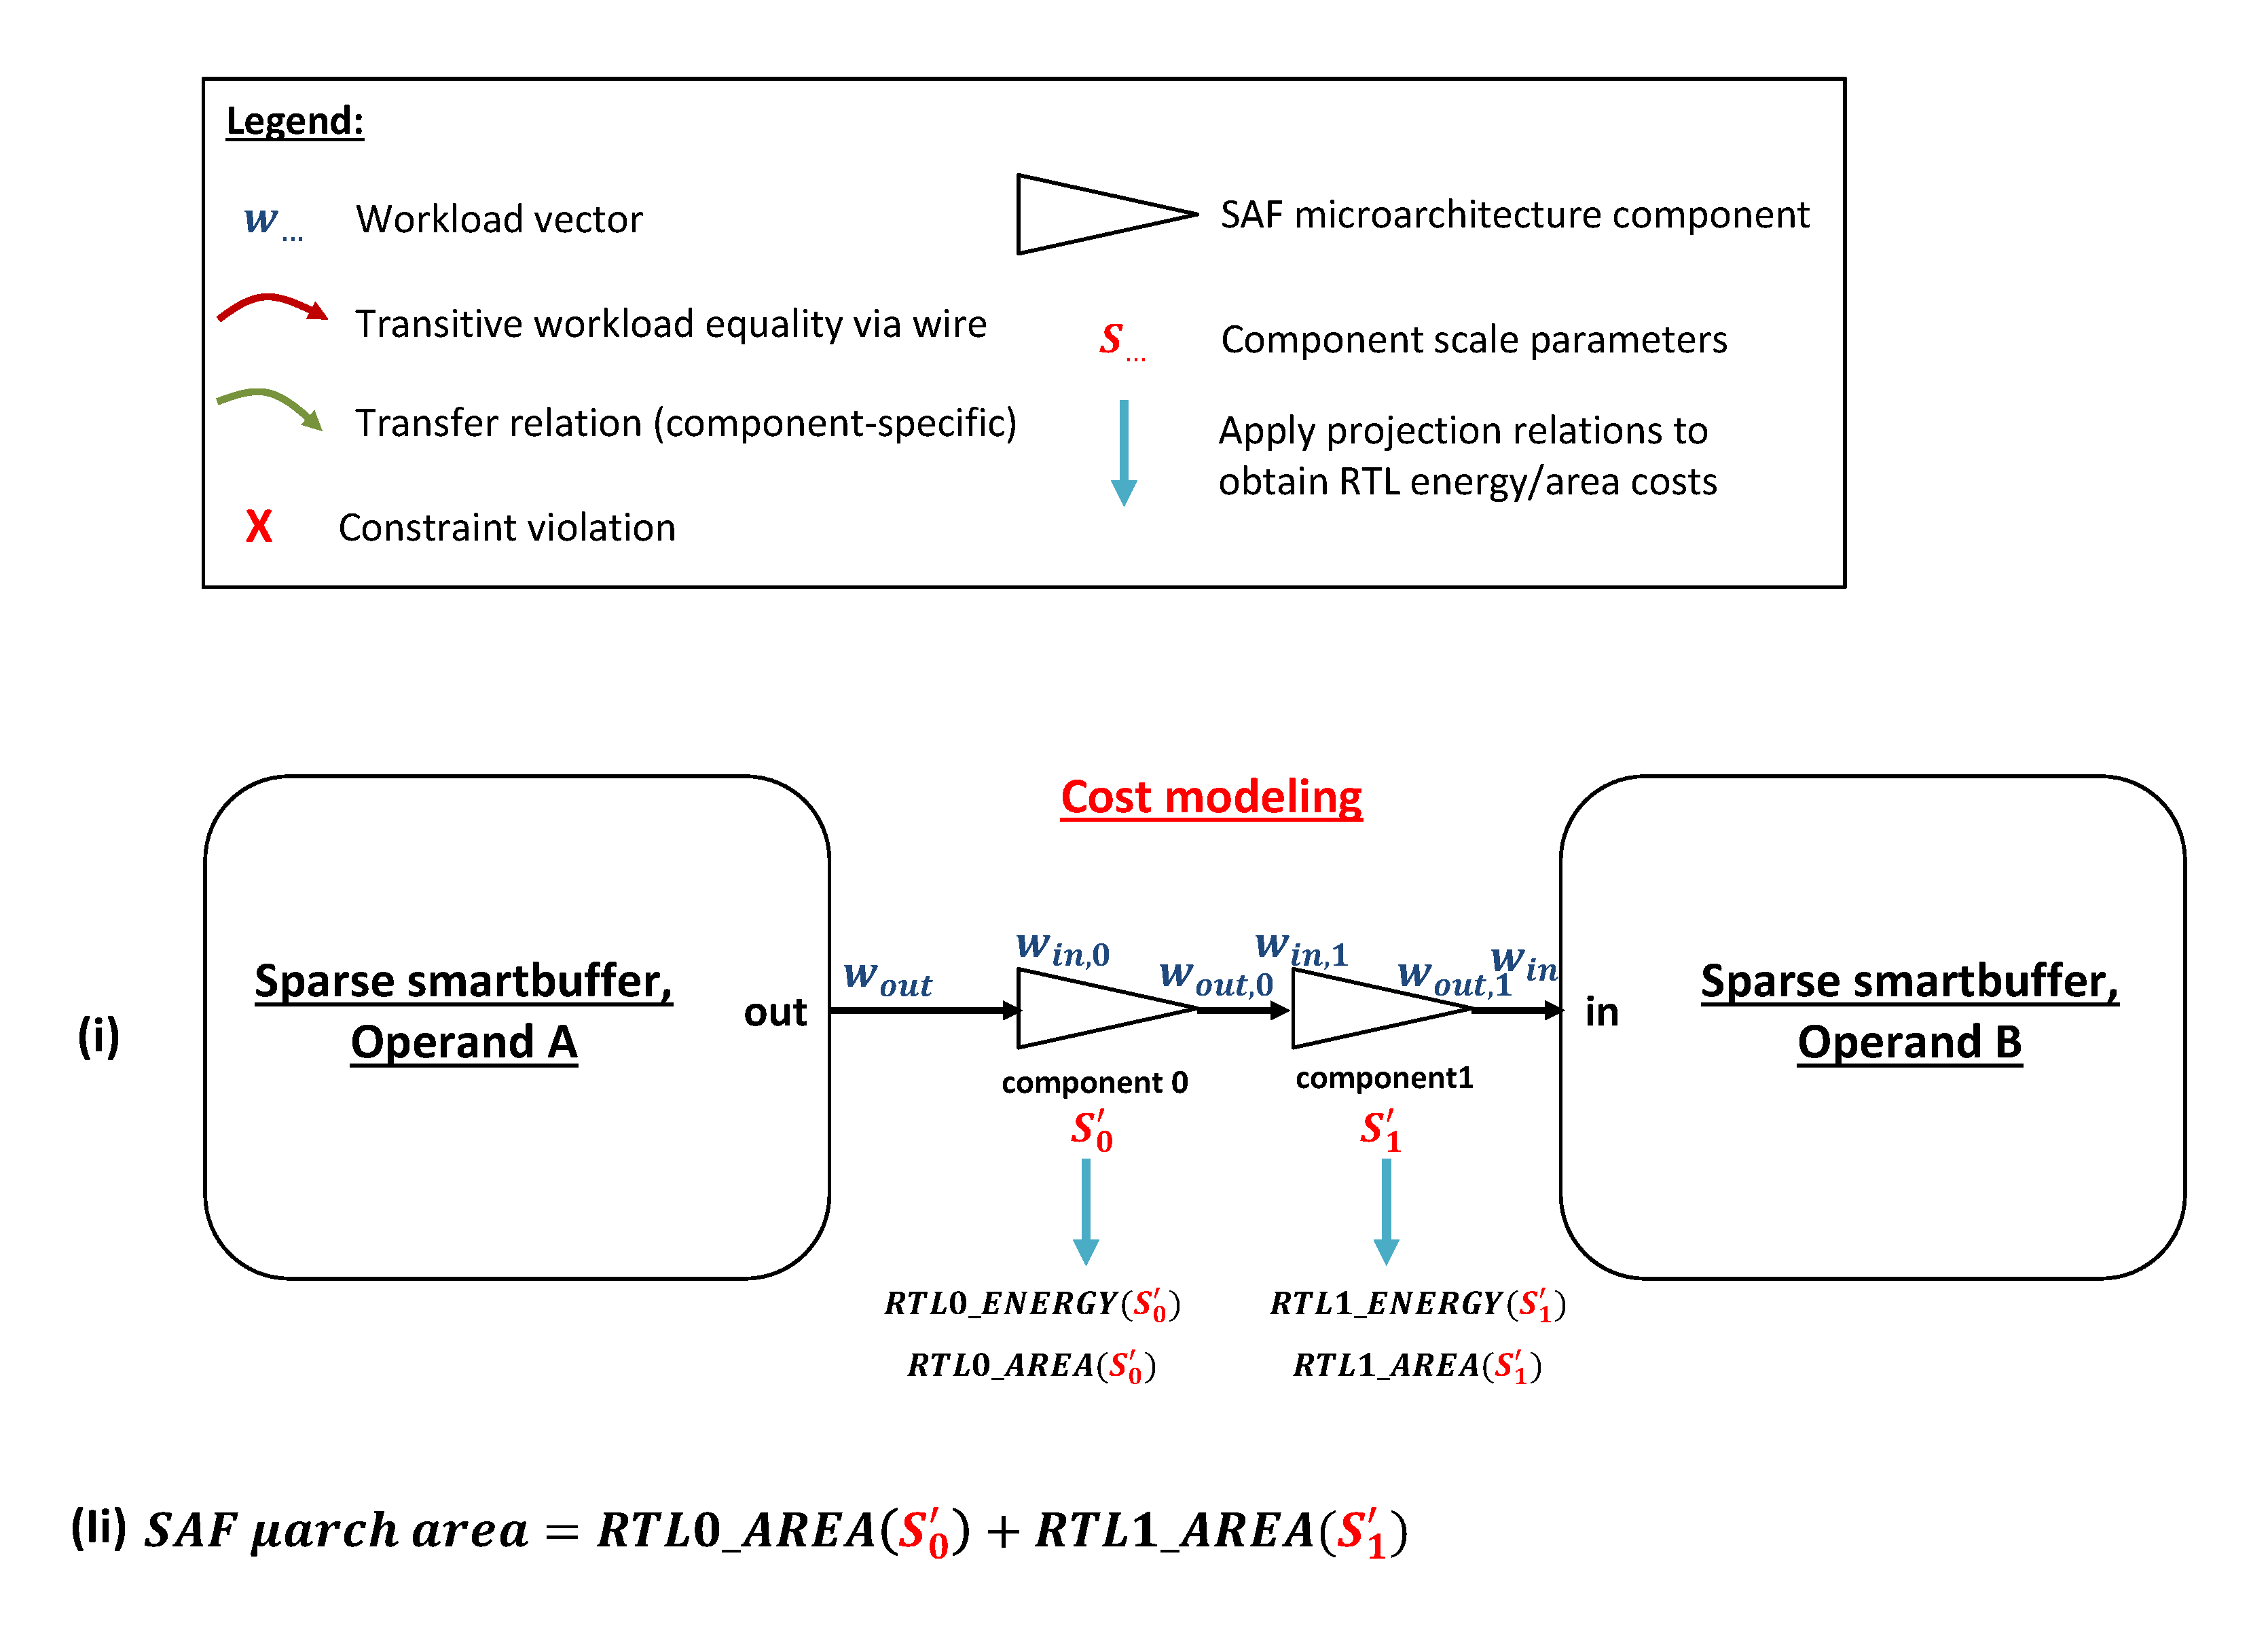
\includegraphics[width=0.8\textwidth]{figures/rtl_objective.pdf}
    \caption{Demonstration of how SAF microarchitecture scale inference makes it possible to derive values for energy and area objective functions.}
    \label{fig:rtl_objective}
\end{figure}

\clearpage

For modeling purposes, a SAF microarchitecture primitive model may be described entirely in terms of:

\begin{itemize}
    \item \textbf{RTL blocks -} A list of RTL modules or ``blocks'' from Chapter~\ref{chapter:rtl} which comprise the component being modeled. Figure~\ref{fig:rtl_objective} reflects that each SAF microarchitecture component may be associated with zero or more characterized RTL components. When the user defines the model of a SAF microarchitecture primitive, they must specify the list of related RTL blocks explicitly.
    \begin{itemize}
        \item \textbf{RTL parameters -} Each RTL block has zero or more parameters which customize the digital logic implementation as a function of the parameter values. RTL parameter values also impact the energy and area cost of a component. The notation for a given RTL parameter is $rtl\_name.param\_name$
        \item \textbf{Example -} A coordinate-payload-format\cite{sparseloop}\cite{szebook} intersection unit\cite{extensor} may (within the context of this work) be constructed out of EXACTLY ONE OF the following RTL blocks defined in Chapter~\ref{chapter:rtl}: a two-fingered intersection unit\cite{extensor}, a skip-ahead intersection unit\cite{extensor}, or a direct-mapped intersection unit.\cite{extensor} (of course the modeling library could be extended to support other options derived from the literature.) The input vectorization parameter of an intersection unit $isect$ would be represented notationally as $isect.md\_in\_vectorization$.
    \end{itemize}
    \item \textbf{Scale parameters -} A set of parameters which determine the SAF microarchitecture primitive's load-handling capability. Figure~\ref{fig:workload_example} shows that each component is associated with a vector $S_x$ of scale parameter values. \textbf{Critically, scale parameters are distinct from taxonomic attributes} - taxonomic attributes are high-level characteristics which reflect choices about algorithm or scaling behavior; once the taxonomic attributes have been specified, \textit{scale parameters represent the low-level design space for sizing RTL blocks in order to satisfy workloads.}
    \begin{itemize}
        \item \textbf{Notation -} $S_x$ is the vector of scale parameters for component $x$.
        \item \textbf{Example -} The scale parameters of a prefix-sum unit are (1) its \textbf{word bitwidth}, and (2) its \textbf{degree of vectorization}. The prefix-sum unit cannot sum a vector which is larger than its vector scale parameter. It cannot correctly sum a vector with words which have more bits than the prefix-sum unit's word bitwidth scale parameter.
    \end{itemize}
    \item \textbf{The component's \textit{constitutive relations} define a unique set of relationships between the workloads applied at each of the component's interface ports, and the parameters of the component's RTL blocks; the constitutive relations should express an intuition about how the component functions.} Constitutive relations are specified at the time when the user writes a SAFTools model. \textbf{The key constitutive relations are:}
    \begin{itemize}
        \item \textbf{Interface constraints.} The interface constraints set \textbf{upper-bounds} on workload at each component input port (i.e. upper-bounds on each dimension of the workload vector at an input port.) This is reflected by Figure~\ref{fig:workload_example}(ii). These upper-bounds are a function of the scale parameter values $S$.
        \begin{itemize}
            \item \textbf{Notation.} $I[S](w_{port0},w_{port1},...)$ is a set of interface constraints on a set of ports' workloads, parameterized by the scale parameters $S$. Typically, $I[S]()$ imposes \textit{upper-bounds}, and upper-bounds increase as $S$ increases along any dimension. \textbf{Critically, component energy/area cost also increases as $S_{comp}$ increases along any dimension.}
            \item \textbf{Corollary.} If a component has scale parameters $S_{comp}$ and the workload applied at $port0$ violates the constraint(s) $I[S_{comp}](w_{port0})$, one can perform ``design-space exploration'' or ``tuning'' of $S_{comp}$ in order to find the minimum-cost $S^\prime_{comp}$ for which $I[S^\prime_{comp}](w_{port0})$ is satisfied by the workload at port0. This is represented in Figure~\ref{fig:workload_example}(ii), where the scale parameters $S_0$ are adjusted to $S^\prime_0$ such that component 0 will support its input workload.
        \end{itemize}
        \item \textbf{Transfer relations.} The transfer relations are \textbf{equations or upper-bound inequalities on output-port workload(s) as a function of input-port workload(s)}; like interface constraints, transfer relations are parameterized by scale parameters. Figure~\ref{fig:workload_example} (iii) and (iv) show how output workload values (or bounds) are derived from input workloads via transfer relations. Transfer relations capture a key intuition that \textbf{SAF microarchitecture primitives frequently exploit forms of filtering or compaction, operations which yield fewer outputs (or fewer \textit{valid outputs}) than inputs.} Critically, this means that if a smartbuffer's output port applies a workload to component 0's input port, and component 0 in turn applies a load to component 1's input port (as is the case in Figure~\ref{fig:workload_example}), the workload at component 1's input port may not be the same as the workload which the smartbuffer imposes on the input port of component 0. Thus, we need transfer relations in order to know how a much workload one component will impose on others.
        \begin{itemize}
            \item \textbf{Notation.} $T[S_{comp}](w_{port\_in0},w_{port\_in1},...)$
            \item \textbf{Example.} Intersecting two compressed sparse coordinate payload fibers, with $C_0$ and $C_1$ non-zero values respectively, necessarily yields an output stream which will contain $C_{out}$ non-zero matching metadata values, where $C_{out} \leq C_0$ and $C_{out} \leq C_1$. Suppose that we know (for sake of simplicity) that $C_{out} = 0.5 C_0$. Then $T[S_{comp}](w_{port\_in0},w_{port\_in1},...)$ is a set containing two relations:

            \[w_{port\_out,pr} \leq 0.5 w_{port\_in0,pr}\]

            \[w_{port\_out,pr} \leq 0.5 w_{port\_in1,pr}\]

            where $w_{port\_out,pr}$, $w_{port\_in0,pr}$ and $w_{port\_in1,pr}$ represent the \textbf{local throughput dimension (mnemonic ``pr'')} of the $port\_out$, $port\_in0$, and $port\_in1$ interfaces, respectively.
            
            \item \textbf{Example.} If two compressed sparse fibers are being intersected, the underlying dense ranks for both fibers necessarily have the same size - and furthermore, the intersected metadata stream at the intersection unit output necessarily also maps back onto the same underlying dense rank. Thus for an intersection unit, the following transfer relations also apply:

            \[w_{port\_out,nc} = w_{port\_in0,nc}\]

            \[w_{port\_out,nc} = w_{port\_in1,nc}\]

            where the $nc$ subscript refers to the dense rank size dimension (mnemonic ``nc'') of each port's workload.
        \end{itemize}
        \item \textbf{Projection relations.} The projection relations allow a SAF microarchitecture primitive's scale parameters to be converted into an analytical model, by adjusting the underlying RTL parameters to match. Projection relations are equations relating RTL parameters to SAF microarchitecture primitive scale parameters.
        \begin{itemize}
            \item \textbf{Notation.} $P[S_{comp}](RTL0,RTL1,...)$
            \item \textbf{Example.} Consider a hypothetical SAF microarchitecture primitive \textit{comp} with with some scale parameter $s \in S_{comp}$, which derives its analytical model from an RTL block \textit{RTL} with a single parameter $p$. Then the projection relations $P[S_{comp}]$ might include

            \[comp.s = RTL.p\]
        \end{itemize}
    \end{itemize}
\end{itemize}

\subsection{Primitive scale inference: solving for scale parameters which satisfy workloads.}

Figure~\ref{fig:workload_example} and Figure~\ref{fig:rtl_objective} summarize the process of \textit{scale inference}, whereby we solve for each SAF microarchitecture primitive's scale parameters $S_x$ where $\{x\}$ is the set of SAF microarchitecture primitive IDs. 

The criteria for valid scale parameters is

\begin{itemize}
    \item All SAF microarchitecture \textit{interface constraints} must be satisfied. If a SAF microarchitecture input is connected to an output wire from a format interface IO bundle, the workload boundary condition associated with that format interface must satisfy the SAF microarchitecture input's interface constraint. If the SAF microarchitecture input is connected to another SAF microarchitecture's output port, the other SAF microarchitecture's output workload must satisfy the SAF microarchitecture input's interface constraint.
    \item For format interface input wires, all \textit{workload boundary conditions} must be satisfied by the SAF microarchitecture output wire connected to the format interface input wire.
\end{itemize}

Scale inference is then a search process over $\{S_x\}$ in order to satisfy the above constraints. Note the following:

\begin{itemize}
    \item SAF microarchitecture primitive interface constraints $I$ and SAF microarchitecture primitive transfer relations $T$ are parameterized by the scale parameters $\{S_x\}$. Thus, adjusting $\{S_x\}$ can (1) make $I$ easier to satisfy by raising upper bounds on workload, or (2) transfer less workload to a downstream component, by adjusting the transfer relation $T$.
    \item Workload boundary conditions associated with format interfaces are immutable.
    \item Projection relations are immutable.
\end{itemize}

The starting-point for scale inference is to flatten all SAF microarchitectures in the entire architecture - i.e., get rid of the higher-level abstractions like SKIP and FMT, and express the microarchitecture entirely in terms of SAF microarchitecture primitives. Having done this, we are left with a graph of all SAF microarchitecture primitives in the architecture, and their interconnections. From this we are able to obtain a large set of relations which define the feasible regions of $\{S_x\}$. And from the projection relations, we are able to define an objective function $f(\{S_x\})$ by mapping scale parameters to RTL parameters, and then looking up characterized RTL metrics based on the parameter values.

This yields a mixed-integer non-linear program (MINLP) for minimizing $f(\{S_x\})$ subject to interface constraints and workload boundary conditions on $\{S_x\}$.

\section{Modeling coordinate-payload intersection units}
\label{sec:c_c_isect_modeling}

Up to this point, this section has been very general. Now, we will show an example of finding transfer relations that are applicable to coordinate-payload bidirectional intersection units.

The difficult part of modeling the transfer relation for coordinate payload intersection units, is determining the relationship between input throughput and output throughput.

The scale parameters of the coordinate payload bidirectional intersection unit are

\begin{itemize}
    \item \textbf{Word width -} The metadata word bitwidth.
    \item \textbf{Input vectorization -} The size of the two metadata vectors being intersected.
    \item \textbf{Pipeline depth -} The depth of the intersection unit's vector pipeline.
\end{itemize}

\begin{figure}[ht]
    \centering
    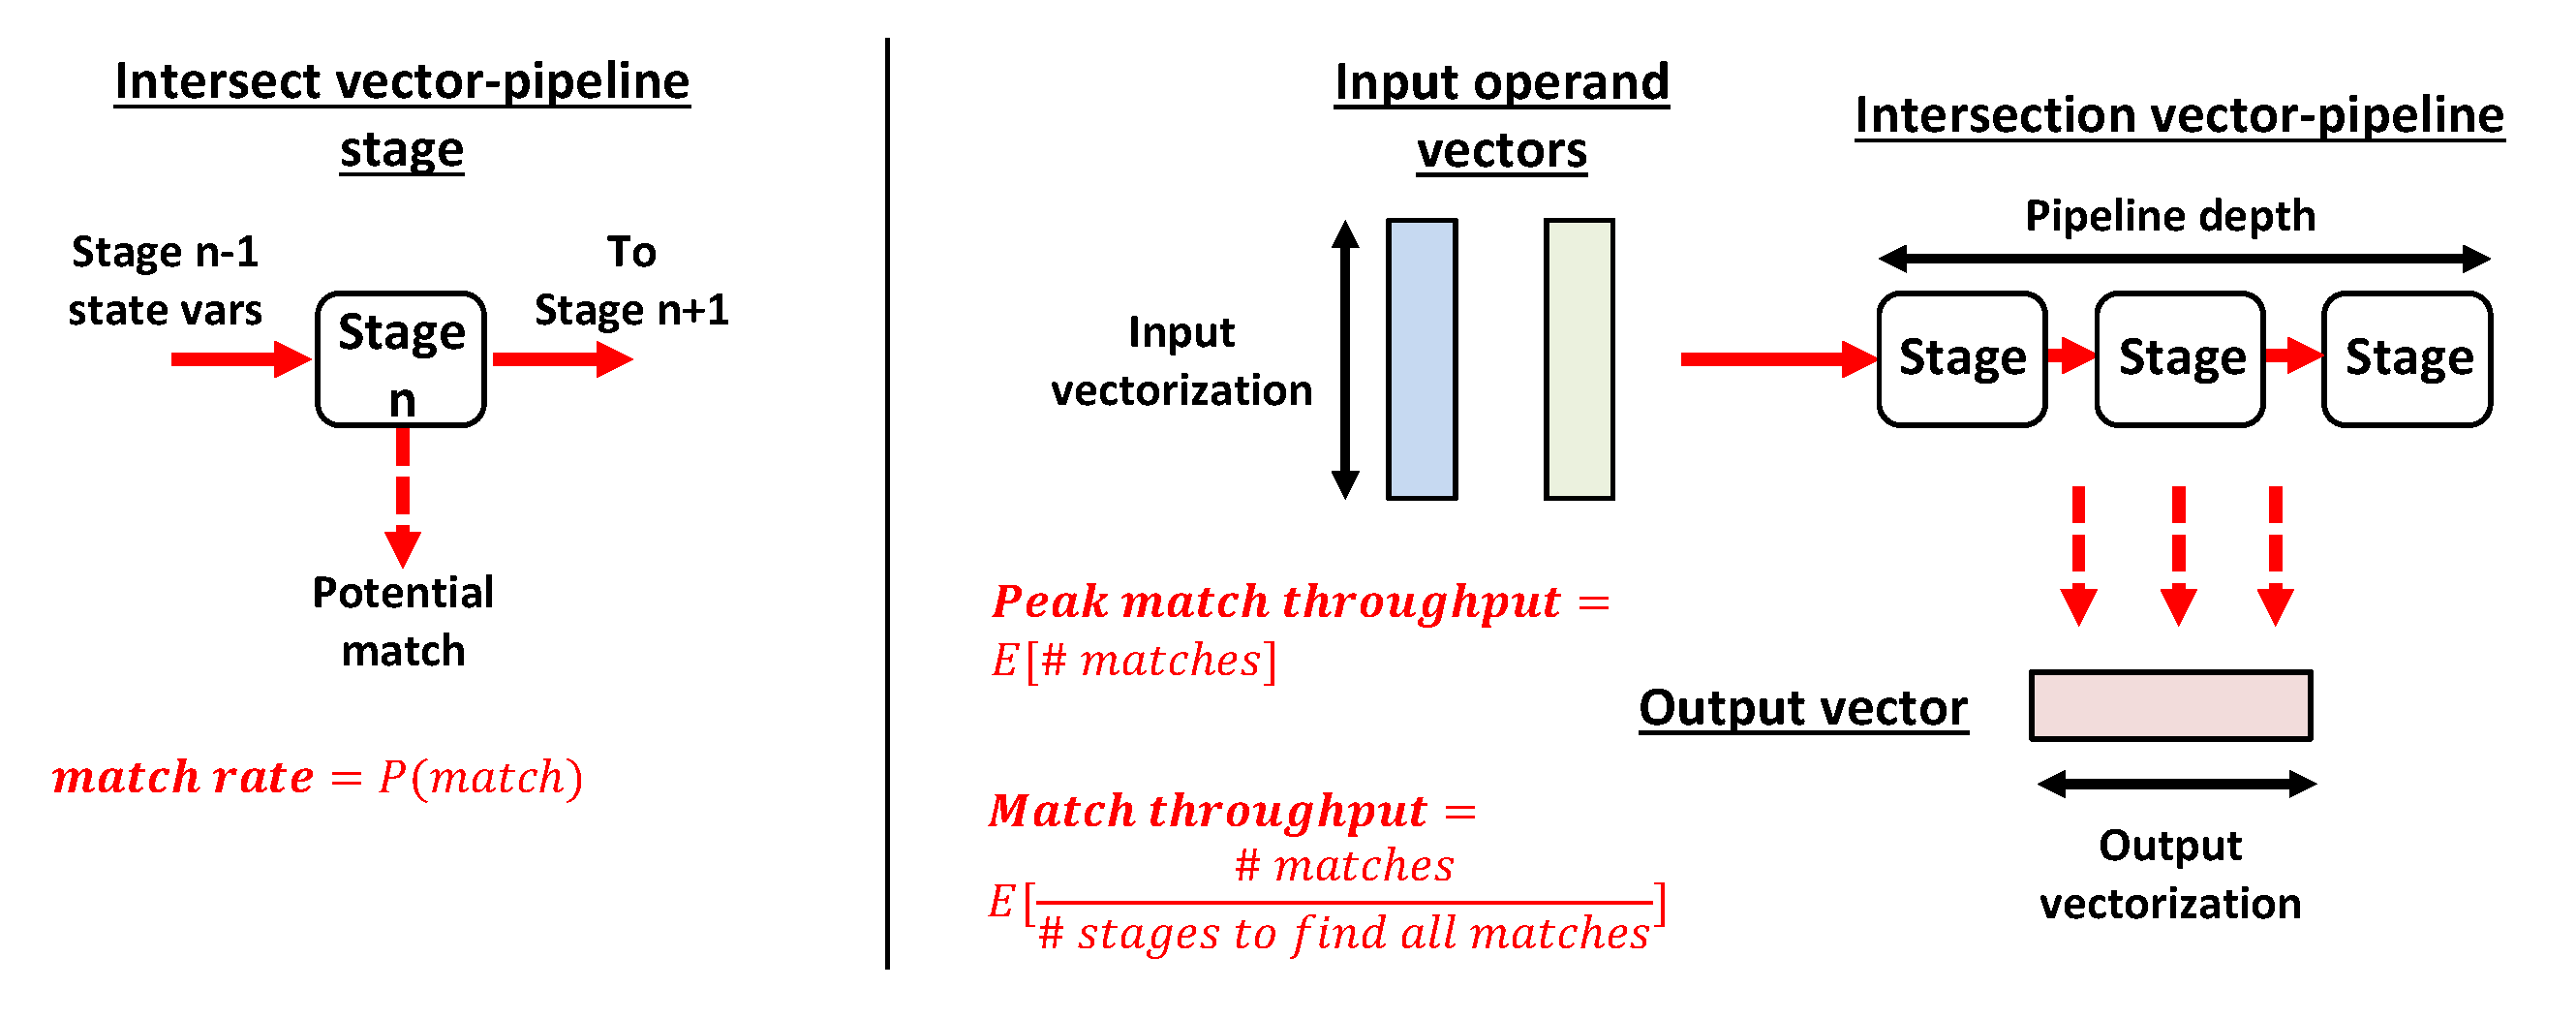
\includegraphics[width=0.95\textwidth]{figures/isect_model.pdf}
    \caption{Diagram of the relationship between the scale parameters of a vector-pipelined intersection unit (vectorization, vector-pipeline depth), and the match throughput.}
    \label{fig:isect_model}
\end{figure}

Figure~\ref{fig:isect_model} summarizes how intersection units are modeled in this work: on average, a pair of vectors will contain a certain number of matches, which is independent of the choice of intersection unit but which does depend on dense rank size, input vectorization, and the sparsity of both operands. The average number of matches thus constitutes an upper limit on the average match rate of the intersection unit i.e. the intersection unit cannot source more matches per cycle, than there are actually existing matches between the two vectors. 

However, the choice of intersection unit affects the probability that a match is found \textit{in a given cycle}; some intersection units have more efficient pipelines. With just a single pipeline stage, this probability of finding a match determines the match throughput at the intersection unit output. With multiple pipeline stages, the match throughput at the intersection unit output is multiplied by the pipeline depth, however the match throughput as already stated cannot exceed the expected number of actually existing matches between the two vectors.

Finding the transfer relation for the intersection unit, reduces to finding the match throughput conditional on the scale parameter values and the operand sparsities. The relationship between these quantities will be affected by the RTL block we choose to implement our intersection unit; in this work the RTL blocks we consider are

\begin{itemize}
    \item ExTensor-like naive two-finger intersection unit\cite{extensor}
    \item ExTensor-like optimized or ``skip-ahead'' intersection unit\cite{extensor}
    \item Direct-mapped intersection unit, which was developed for this work.
\end{itemize}

Note that direct-mapped intersect unit finds 100\% of matches within a single cycle, at the cost of increased area; other intersection unit types may require more cycles or more pipeline stages in order to find all matches.

To solve this problem, three cycle-accurate model were implemented, one for each intersection unit. These cycle-accurate models simulate the number of cycles required to intersect two vectors using a single-stage intersection pipeline and assuming that the intersection process entails making chained calls to the same vectorized intersection hardware until the process is complete. Each simulator is run in a testbench, which simulates the process of breaking two fibers into vectors matching the intersection unit's input vectorization, and performing intersections vector-by-vector until both fibers have been intersected in their entirety yielding an output list of coordinate metadata for all of the matches.

A simple machine learning model was implemented, combining a rule-based decision tree in which each tree leaf is associated with a different 3rd-order polynomial model. The inputs to the machine learning model are type of intersection unit, dense rank size, sparsity of both operand fibers, and degree of input vectorization of the intersection unit. The output is a prediction of the number of cycles required to intersect both fibers in their entirety. The cycle-accurate simulator was used to generate train and test datasets; the machine learning model was fitted to the training dataset and then evaluated on the unseen data in the test dataset. Figure~\ref{fig:isect_model_fl8_vl4} shows how the predicted match throughput values for the intersection unit compare to the actual values generated by the cycle accurate simulator; additional analysis of this transfer relation model can be found in Appendix~\ref{appendix:app_intersection_modeling}. Section~\ref{chapter:evaluation} will discuss the performance of this machine learning model.

\begin{figure}[ht]
    \centering
    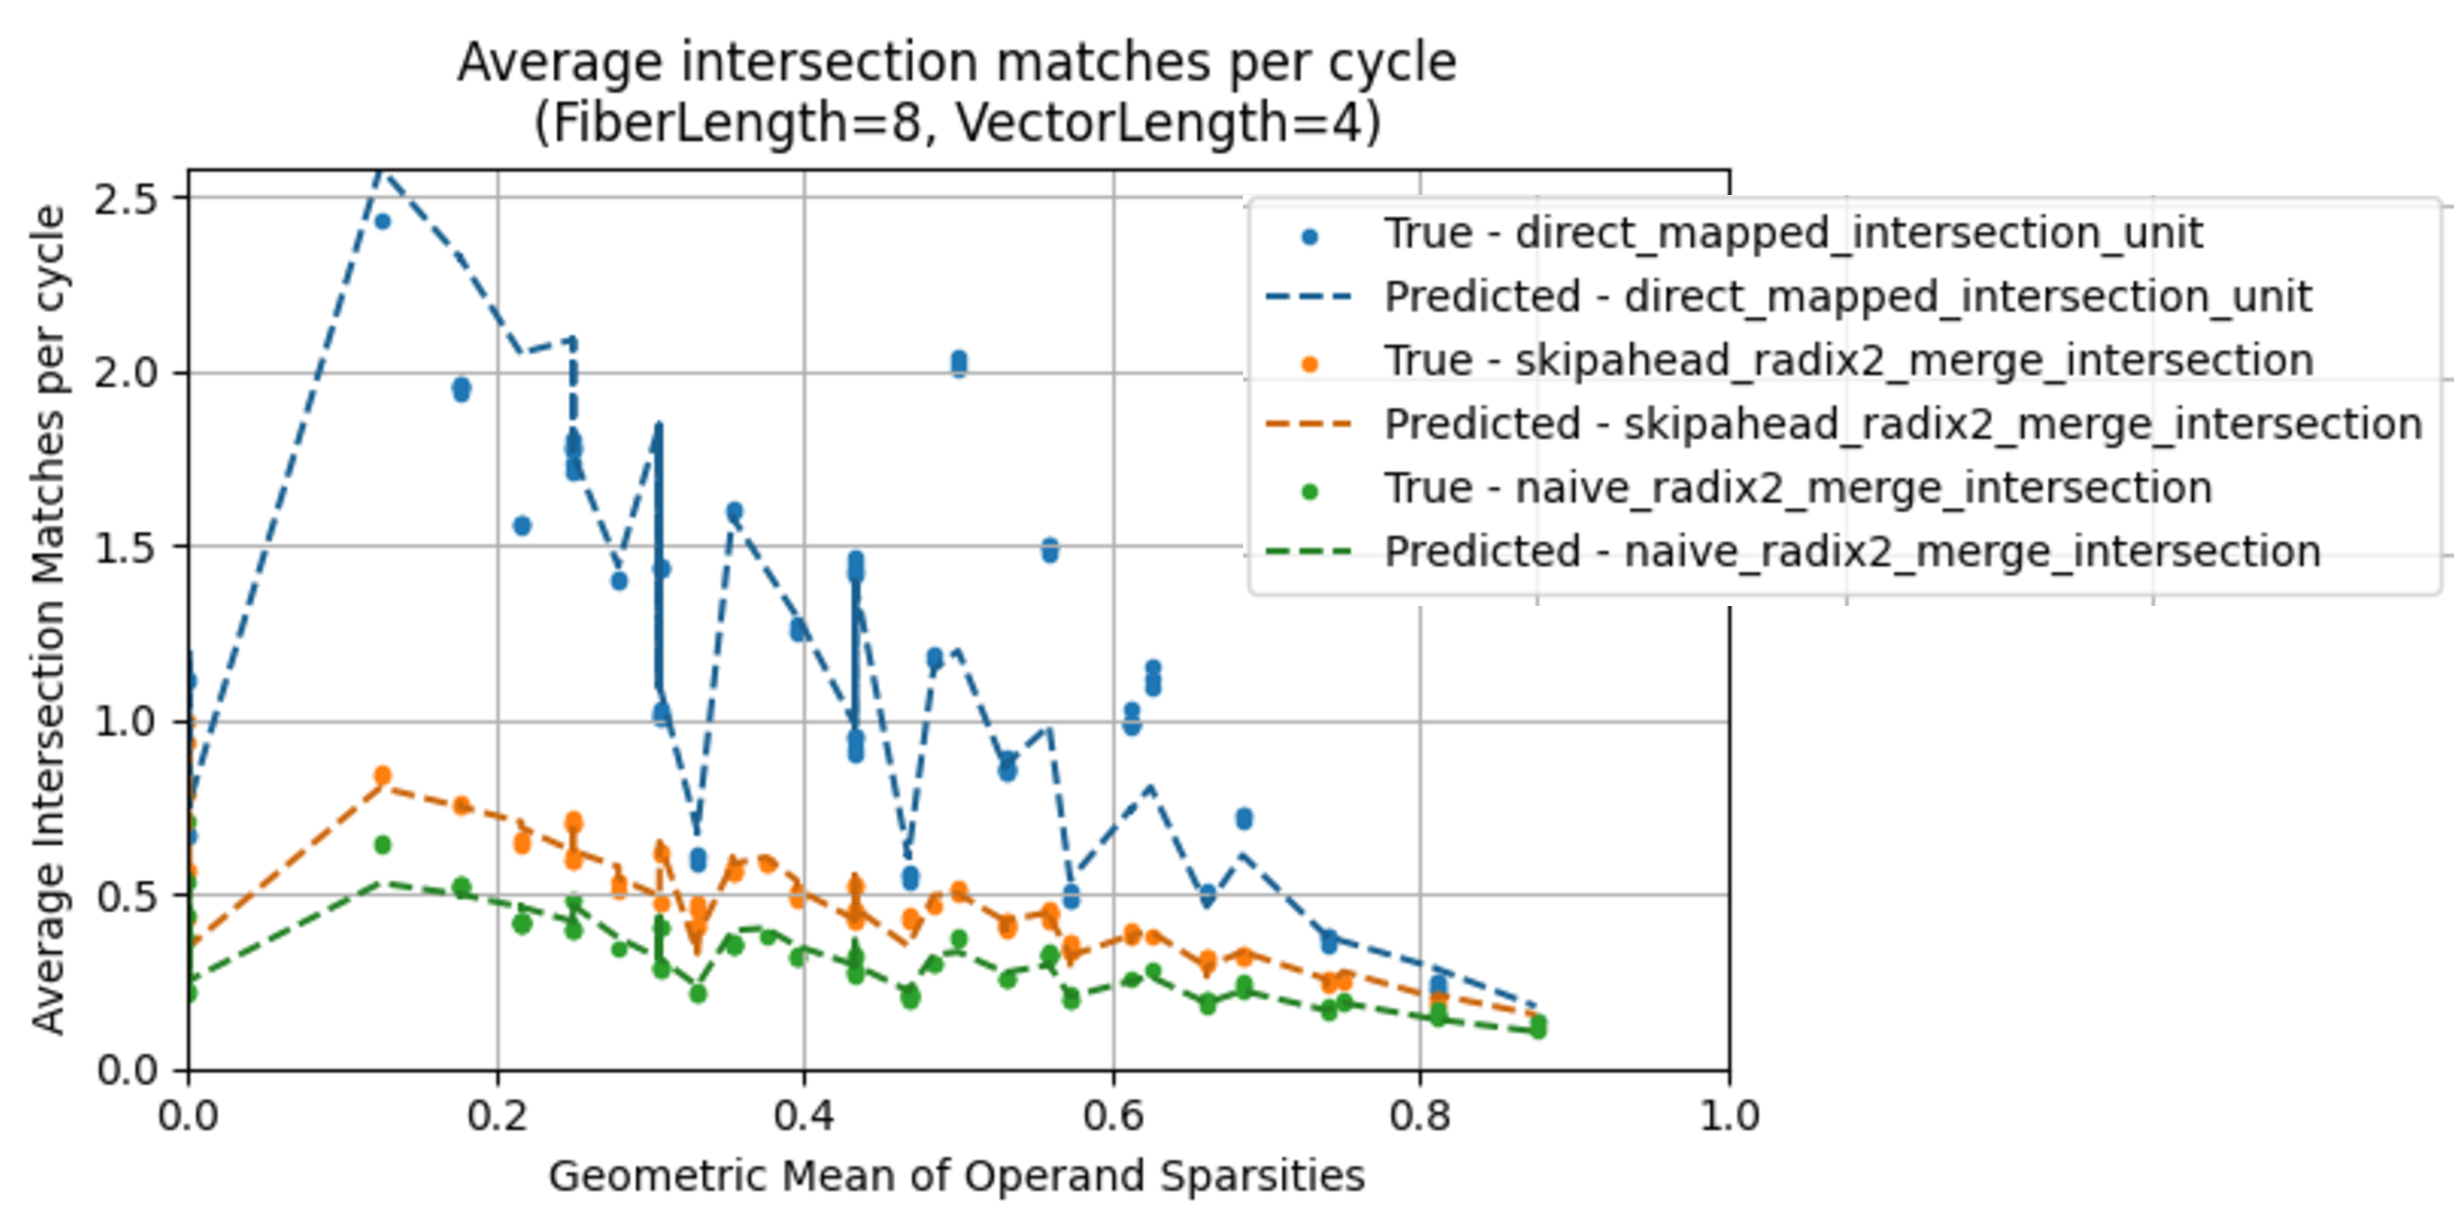
\includegraphics[width=0.95\textwidth]{figures/isect_model_fl8_vl4.pdf}
    \caption{Comparison of match throughput with respect to sparsity (geomean) for fiber size 8 and input vectorization 4. The predicted match throughput values from the analytical model developed for this work, are overlaid on simulated measurements from the intersection unit cycle accurate simulators. Additional analysis of this model is provided in Appendix~\ref{appendix:app_intersection_modeling}}
    \label{fig:isect_model_fl8_vl4}
\end{figure}

Note that the machine learning model relates the input workload - i.e. fiber sparsity, dense rank size - to the output workload - i.e. match throughput. Thus this machine learning model is the transfer relations for the bidirectional intersection SAF microarchitecture primitive. By passing this machine learning model through a computer algebra system, it was possible to obtain a symbolic representation of the transfer relation. This symbolic representation was integrated into the model definition.